% Polska wersja artykułu qaoa_gcmm — pełne tłumaczenie 1:1 (bez skrótów).
% Wiążąca jest wersja angielska (main.tex). Kompilacja: xelatex wersja_pl.tex
% Rysunki są reużywane z figures/ — etykiety na diagramach obwodów i na wykresie
% pozostają angielskie, bo są wkompilowane w pliki PDF.
\documentclass[11pt,a4paper]{article}
\usepackage{fontspec}
\usepackage{polyglossia}
\setdefaultlanguage{polish}
\usepackage{amsmath,amssymb}
\usepackage{booktabs}
\usepackage{graphicx}
\usepackage{xcolor}
% przelacznik z main.tex; w wersji roboczej PL pokazujemy prawdziwe autocytowania
\newif\ifblind\blindfalse
\usepackage[margin=2.3cm]{geometry}
\usepackage{enumitem}
\setlist{nosep}
\usepackage{microtype}
\emergencystretch=3em
\hfuzz=1pt
\usepackage{hyperref}
\hypersetup{colorlinks=true, linkcolor=blue!55!black, citecolor=blue!55!black,
            urlcolor=blue!55!black}
\providecommand{\doi}[1]{\href{https://doi.org/#1}{\texttt{doi:\detokenize{#1}}}}
\newcommand{\keywords}[1]{\par\medskip\noindent\textbf{Słowa kluczowe:} #1}

\title{Bramkowe kwantowe przeszukiwanie sąsiedztwa dla permutacyjnego
  problemu przepływowego przez QAOA o ustalonych kątach\\[2pt]
  \large Pełne tłumaczenie robocze -- wiążąca jest wersja angielska (main.tex)}
\author{Remigiusz Wojewódzki \and Wojciech Bożejko\\
  \small Katedra Sterowania i Obliczeń Kwantowych, Wydział Informatyki
  i Telekomunikacji,\\ \small Politechnika Wrocławska, Wrocław, Polska}
\date{Tłumaczenie z 4.10.2026 -- cel wydawniczy: GCMM 2026, sesja SS3
  (Springer LNME/LNNS)}

\begin{document}
\maketitle

\begin{abstract}
\noindent
Permutacyjny problem przepływowy (PFSP) to kanoniczny problem szeregowania
klasy NP-trudnej, w którym solvery oparte na przeszukiwaniu lokalnym zużywają
większość wysiłku na ocenianie ruchów sąsiedztwa. Niedawne prace przeniosły tę
ocenę na kwantowe annealery, odwzorowując sąsiedztwa jako problemy QUBO, lecz
paradygmat bramkowy -- przy całej swojej elastycznej łączności -- pozostaje
w szeregowaniu w znacznej mierze niezbadany. Niniejszy artykuł wprowadza
framework bramkowy, który ocenia sąsiedztwa PFSP za pomocą kwantowego
przybliżonego algorytmu optymalizacyjnego (QAOA) wbudowanego w klasyczne
metaheurystyki iterowanego przeszukiwania lokalnego i symulowanego wyżarzania.
Reużywamy kodowania QUBO typu swap-selection z linii annealingowej, tak że
jedna macierz problemu napędza albo annealer, albo obwód QAOA, i przyjmujemy
QAOA o ustalonych kątach, których parametry wariacyjne są preoptymalizowane
offline; na sprzęcie każdy ruch kosztuje wówczas jedno wykonanie obwodu, co
utrzymuje metodę w granicach ograniczeń NISQ. Formułujemy wszystkie cztery
struktury sąsiedztw (Adjacent, Fibonacci, Dynasearch, Motzkin) i analizujemy,
jak gęstość ich grafów konfliktów rządzi głębokością obwodu po skompilowaniu
QUBO na sprzęt nadprzewodnikowy -- od kraty heavy-hex do gwiazdy sprzężonej
rezonatorem. Głębokość przyjmuje rolę, jaką na annealerach odgrywa pojemność
embeddingu i daje to samo uszeregowanie wykonalności z innego, zakorzenionego
w kompilacji powodu, a dekompozycja okienkowa poskramia gęste sąsiedztwa.
Pomiary na trzech procesorach rozdzielają dwa reżimy: sąsiedztwa, których
obwody pozostają krótkie, zwracają ten sam makespan na urządzeniu heavy-hex
ze 156 kubitami i na urządzeniu z rezonatorem o 16 kubitach, instancja po
instancji, podczas gdy najgłębsze obwody przesuwają się między mapami
sprzężeń. Artykuł przedstawia metodykę oceny, raportuje to wykonanie
i formułuje pozostające otwarte wyzwania.
\keywords{optymalizacja kombinatoryczna, QUBO, metaheurystyki, symulowane
  wyżarzanie, kompilacja obwodów na sprzęt nadprzewodnikowy, NISQ}
\end{abstract}

% =====================================================================
\section{Wstęp}
\label{sec:intro}
Permutacyjny problem przepływowy (PFSP) należy do najszerzej badanych
problemów NP-trudnych w szeregowaniu produkcji. Dla $n$ zadań, które muszą
zostać wykonane w tej samej kolejności na $m$ maszynach, zadaniem jest
znalezienie jednej permutacji zadań minimalizującej makespan $C_{\max}$, czyli
czas zakończenia ostatniego zadania na ostatniej maszynie. Ponieważ liczba
permutacji rośnie silniowo, metody dokładne ograniczają się do małych
instancji, a praktyczne solvery opierają się na metaheurystykach
przeszukiwania lokalnego, takich jak iterowane przeszukiwanie lokalne,
symulowane wyżarzanie i przeszukiwanie z zakazami. Metody te zużywają
przeważającą większość czasu działania na jednej operacji wewnętrznej:
ocenianiu ruchów sąsiedztwa, by zdecydować, gdzie zrobić następny krok. Koszt
tej oceny, powtarzanej miliony razy w trakcie przeszukiwania, jest dominującym
wąskim gardłem obliczeniowym i naturalnym celem przyspieszania.

Niedawna linia prac przenosi tę ocenę na sprzęt kwantowy, odwzorowując każde
sąsiedztwo jako problem kwadratowej nieograniczonej optymalizacji binarnej
(QUBO) i rozwiązując go na kwantowym annealerze. Annealer wybiera, w jednym
wywołaniu, podzbiór ruchów, które wspólnie poprawiają makespan bez wchodzenia
ze sobą w konflikt, a klasyczna metaheurystyka rusza dalej ze zwróconej
permutacji. Paradygmat bramkowy pozostał jednak w szeregowaniu niemal
nietknięty, mimo że oferuje programowalne obwody, trasowanie do dowolnych par
kubitów i stale rosnący dostęp przez platformy chmurowe, takie jak IBM
Quantum. Pytanie, na które odpowiada ten artykuł, brzmi: czy ten sam pomysł
sąsiedztwa-jako-QUBO da się przenieść z annealera na urządzenie bramkowe i co
się przy tym zmienia.

Niniejszy artykuł wprowadza framework bramkowy, który ocenia sąsiedztwa PFSP
za pomocą kwantowego przybliżonego algorytmu optymalizacyjnego (QAOA)
wbudowanego w klasyczne iterowane przeszukiwanie lokalne i symulowane
wyżarzanie. Framework reużywa kodowania QUBO typu swap-selection z linii
annealingowej, tak że jedna macierz problemu napędza albo annealer, albo obwód
QAOA, a oba paradygmaty są porównywane na identycznych instancjach. Aby
utrzymać metodę w granicach wykonalności na zaszumionym sprzęcie średniej
skali, przyjmujemy QAOA o ustalonych kątach, w którym parametry wariacyjne są
preoptymalizowane offline i następnie zamrożone, co redukuje koszt online do
jednego wykonania obwodu na ruch -- tego samego budżetu, jaki zużywa annealer.
Formułujemy wszystkie cztery struktury sąsiedztw używane przez linię
annealingową i analizujemy, jak gęstość ich grafów konfliktów rządzi
głębokością obwodu po skompilowaniu QUBO na sprzęt nadprzewodnikowy, na mapach
sprzężeń sięgających od kraty heavy-hex do gwiazdy sprzężonej rezonatorem.
Naszą centralną obserwacją jest to, że ta głębokość odgrywa rolę, jaką na
annealerze odgrywa pojemność embeddingu: daje to samo uszeregowanie
wykonalności sąsiedztw z innego, zakorzenionego w kompilacji powodu,
a dekompozycja okienkowa poskramia gęste sąsiedztwa tak samo jak na
annealerze.

Praca ta zajmuje się metodyką oceny i jej analizą, a nie wielkoskalowym
benchmarkiem sprzętowym, i dwa ograniczenia uzasadniają to zawężenie. Obecne
urządzenia bramkowe są zaszumione i płytkie, więc obwód nieco zbyt głęboki
zwraca próbki niemal losowe. Istotna jest zatem wiedza z wyprzedzeniem, które
sąsiedztwa kompilują się do płytkich obwodów. Dostęp chmurowy jest ponadto
rozliczany w minutach na miesiąc, co wyklucza wiele wykonań eksploracyjnych,
jakich wymagałby wariacyjny QAOA, i czyni projekt offline o ustalonych kątach
koniecznością. Framework już teraz daje wyniki, które przenoszą się poza jedno
urządzenie. Jedna macierz QUBO typu swap-selection napędza zarówno annealer,
jak i obwód QAOA, więc sąsiedztwa i ich kary przechodzą bez zmian, a zmienia
się tylko backend solvera. Argument o głębokości daje następnie regułę wyboru
sąsiedztw niezależną od sprzętu. Sąsiedztwo, które mieści się w łączności
annealera, kompiluje się też do płytkiego obwodu bramkowego. Symulacja wchodzi
tylko raz, offline, aby ustalić kąty QAOA; każdy raportowany przez nas wynik
jest zmierzony na procesorach kwantowych.

% =====================================================================
\section{Przegląd literatury}
\label{sec:related}
Permutacyjny problem przepływowy służy jako poligon dla algorytmów szeregowania
od czasu, gdy Taillard udostępnił instancje benchmarkowe pozostające
w standardowym użyciu do dziś. Problem jest silnie NP-trudny już przy trzech
lub więcej maszynach, co ustalili Garey, Johnson i Sethi, i dlatego praktyczne
solvery opierają się na heurystykach. Wśród heurystyk konstrukcyjnych metoda
Nawaza, Enscore'a i Hama jest nadal uznawana za najsilniejszą w swojej klasie
i stanowi zwykły punkt startowy dla przeszukiwania lokalnego. Ruiz i Maroto
porównali duży zbiór heurystyk i metaheurystyk dla kryterium makespanu
i potwierdzili, że iterowane przeszukiwanie lokalne oraz symulowane wyżarzanie
należą do najskuteczniejszych podejść. Te dwie metaheurystyki, które w naszym
frameworku są gospodarzami podprocedury kwantowej, wywodzą się z tej
literatury: symulowane wyżarzanie wprowadzili jako ogólną metodę
optymalizacyjną Kirkpatrick, Gelatt i Vecchi, a iterowane przeszukiwanie
lokalne sformalizowali później Lourenço, Martin i Stützle. Siła takich metod
zależy od tego, jak duże sąsiedztwo potrafią przeszukać w każdym kroku. Ahuja,
Ergun, Orlin i Punnen dokonali przeglądu przeszukiwania bardzo
wielkoskalowych sąsiedztw, w którym sąsiedztwo rozmiaru wykładniczego bada się
w czasie wielomianowym. Congram, Potts i van de Velde wprowadzili dynasearch,
który używa programowania dynamicznego do zastosowania kilku niezależnych
ruchów wymiany w jednym kroku i daje nazwę badanemu tu sąsiedztwu Dynasearch.

Nowszy kierunek zastępuje klasyczną ocenę tych sąsiedztw podprocedurą
kwantową, kodując każde sąsiedztwo jako QUBO, którego rozwiązanie wybiera
zbiór zgodnych poprawiających wymian. Jedno badanie sformułowało klasyczne
i kwantowe wersje kilku sąsiedztw przepływowych i porównało je wewnątrz
iterowanego przeszukiwania lokalnego oraz symulowanego wyżarzania. Praca
towarzysząca wprowadziła sąsiedztwo Motzkina, którego struktura
nieprzecinających się par daje rzadszy graf konfliktów niż alternatywy oparte
na nakładaniu. Trzecia uczyniła podejście skalowalnym przez okienkową
dekompozycję QUBO, która utrzymuje każdy podproblem w granicach łączności
annealera. Niniejsza praca przyjmuje te kodowania QUBO bez zmian i bada ich
zachowanie na sprzęcie bramkowym.

Odwzorowanie problemów kombinatorycznych na kwadratową formę binarną opiera
się na modelu Isinga, a Lucas skatalogował sformułowania Isinga dla szerokiego
zakresu problemów NP, ograniczając przy tym liczbę spinów wymaganą przez
każdy z nich. Kwantowe wyżarzanie jest procesem fizycznym, do którego te
sformułowania celują; Kadowaki i Nishimori wprowadzili je jako metodę pola
poprzecznego do sprowadzania układu Isinga do stanu podstawowego. Na realnym
sprzęcie Venturelli, Marchand i Rojo zrealizowali szeregowanie gniazdowe na
annealerze D-Wave i zaraportowali zarówno jego obietnicę, jak i ograniczenia
embeddingu, które limitują rozmiar problemu.

Bramkowym odpowiednikiem kwantowego wyżarzania dla optymalizacji jest kwantowy
przybliżony algorytm optymalizacyjny Farhiego, Goldstone'a i Gutmanna, który
naprzemiennie stosuje warstwy kosztu i miksera, a ich kąty są dostrajane tak,
by zminimalizować funkcję celu. Zhou, Wang, Choi, Pichler i Lukin
przeanalizowali jego krajobraz optymalizacyjny na urządzeniach bliskiego
horyzontu i stwierdzili, że dobre kąty układają się w regularny wzorzec,
a nie rozpraszają po przestrzeni parametrów. Wurtz i Lykov zamienili tę
regularność na hipotezy o ustalonych kątach, dostarczające niemal optymalnych
parametrów bez dostrajania pod instancję, a Galda, Liu, Lykov, Alexeev i Safro
pokazali, że kąty optymalne przenoszą się między grafami o wspólnej strukturze
lokalnej. Te wyniki razem umożliwiają offline'owy projekt o ustalonych kątach
w naszym frameworku. Najbliższą pracą bramkową o szeregowaniu jest praca
Amaro, Rosenkranza, Fitzpatricka, Hirano i Fiorentiniego, którzy uruchomili
kilka wariacyjnych heurystyk kwantowych, w tym QAOA, na małej instancji
szeregowania gniazdowego i uznali zbieżność na obecnym sprzęcie za trudną.
Nasze kodowanie na poziomie sąsiedztwa utrzymuje każdy obwód małym, co
właśnie czyni podejście o ustalonych kątach praktycznym tam, gdzie
sformułowanie end-to-end napotyka trudności.

Sam sprzęt decyduje, które obwody dadzą się w ogóle wykonać. Preskill
scharakteryzował reżim zaszumionych urządzeń kwantowych średniej skali,
w którym szum ostro ogranicza głębokość wiarygodnego obwodu. Procesory
nadprzewodnikowe IBM są zbudowane na kracie heavy-heksagonalnej Chamberlanda,
Zhu, Yodera, Hertzberga i Crossa, która redukuje kolizje częstotliwości za
cenę rzadkiej łączności kubitów. Głębokość obwodu po kompilacji przyjmuje
zatem rolę, jaką na annealerze odgrywa pojemność embeddingu, i to jest
związek, który rozwija niniejszy artykuł.

% =====================================================================
\section{Metodyka badań}
\label{sec:method}

Nasz framework nie dotyka klasycznej metaheurystyki i zastępuje wyłącznie
oracle oceniające sąsiedztwo bramkową podprocedurą kwantową. Każda ocena ruchu
jest odwzorowywana jako instancja QUBO, mapowana na hamiltonian Isinga
i rozwiązywana w przybliżeniu obwodem QAOA o ustalonych kątach. Odzwierciedla
to linię prac annealingowych: jedno QUBO typu swap-selection napędza albo
kwantowy annealer, albo bramkowy obwód QAOA, więc zmienia się tylko backend
solvera, a oba paradygmaty są porównywane na identycznych instancjach.
Podprocedura kwantowa jest wbudowana, bez zmian, w tych samych gospodarzy --
iterowane przeszukiwanie lokalne i symulowane wyżarzanie -- których używa
linia annealingowa.

\subsection{Kodowanie QUBO typu swap-selection}
\label{subsec:qubo}
Reużywamy kodowania swap-selection z linii annealingowej. Sąsiedztwo dostarcza $K$
kandydatów na wymianę, a zmienna binarna $x_k=1$, dla $k=1,\dots,K$, oznacza,
że kandydat $k$ zostaje zastosowany do bieżącej permutacji. Wybór podzbioru zgodnych wymian zapisuje się jako minimalizację
formy kwadratowej
\begin{equation}
  \min_{\mathbf{x}\in\{0,1\}^{K}}\
  \mathbf{x}^{\mathsf T} Q\,\mathbf{x},
  \label{eq:qubo}
\end{equation}
gdzie $Q_{kk}=\delta_k$, dla $k=1,\dots,K$, jest zmianą makespanu wywołaną
wymianą $k$, obliczaną w czasie $O(1)$ przez dekompozycję Head--Tail. Macierz
jest górnotrójkątna, więc dla $1\le k<l\le K$ wyraz $Q_{kl}$ równa się
$\lambda$, gdy kandydaci $k$ i $l$ kolidują, a zero w przeciwnym razie,
i każda kolidująca para jest karana raz. Kara
\begin{equation}
  \lambda \;=\; \sum_{k=1}^{K}\lvert\delta_k\rvert \;+\; 1
  \label{eq:penalty}
\end{equation}
dominuje funkcję celu, więc każde rozwiązanie wybierające dwie kolidujące
wymiany jest droższe niż dowolne rozwiązanie dopuszczalne. Kodowanie one-hot
dla Adjacent jest wyjątkiem. Tam koliduje każda para, więc kara wchodzi także
na przekątną, z $Q_{kk}=\delta_k-P$ i $Q_{kl}=2P$ dla $k<l$, gdzie
$P=2\max_{k}\lvert\delta_k\rvert+1$. Wzorzec karanych
par jest odciskiem palca sąsiedztwa (podrozdział~\ref{subsec:neigh}). Macierz
$Q$ w~\eqref{eq:qubo} jest tą samą macierzą, którą zgłoszono do kwantowego
annealera w pracy towarzyszącej; różni się jedynie solver, który po niej
następuje.

\subsection{Od QUBO do obwodu QAOA}
\label{subsec:circuit}
Zamiana zmiennych $Z_k=2x_k-1$, czyli $x_k=(1+Z_k)/2$, przekształca
QUBO~\eqref{eq:qubo} w isingowski hamiltonian kosztu
\begin{equation}
  H_C \;=\; \sum_{i=1}^{K} h_i Z_i \;+\; \sum_{1\le i<j\le K} J_{ij} Z_i Z_j
  \;+\; \mathrm{const},
  \label{eq:ising}
\end{equation}
gdzie $Z_i$ i $X_i$ są operatorami Pauliego $Z$ i $X$ działającymi na kubit
$i$, po jednym kubicie na kandydata na wymianę, a pola liniowe $h_i$ oraz
sprzężenia $J_{ij}$ wynikają bezpośrednio z wyrazów macierzy $Q$. QAOA o głębokości $p$ przygotowuje stan
sparametryzowany
\begin{equation}
  \lvert\gamma,\beta\rangle \;=\;
  \Bigl(\textstyle\prod_{l=1}^{p}
        e^{-i\beta_l H_M}\,e^{-i\gamma_l H_C}\Bigr)
  \lvert +\rangle^{\otimes K},
  \qquad H_M=\sum_{i=1}^{K} X_i,
  \label{eq:qaoa}
\end{equation}
z mikserem pola poprzecznego $H_M$. Obwód ma $p$ warstw i dwa kąty na warstwę,
$\gamma_l$ dla ewolucji kosztu i $\beta_l$ dla miksera, które optymalizujemy
po $\gamma_l\in[0,\pi]$ i $\beta_l\in[0,\pi/2]$. Dla $p=1$ każda warstwa
kompiluje się do bramek elementarnych. Początkowa warstwa bramek Hadamarda wprowadza rejestr
w równą superpozycję po wszystkich wyborach ruchów. Ewolucja kosztu
$e^{-i\gamma H_C}$ jest realizowana jako rotacja jednokubitowa
$R_Z(2\gamma h_i)$ na każdej zmiennej wraz z rotacją dwukubitową
$R_{ZZ}(2\gamma J_{ij})$ na każdej sprzężonej parze, a mikser
$e^{-i\beta H_M}$ jako rotacja $R_X(2\beta)$ na każdym kubicie. Próbkowanie
obwodu i wzięcie najczęstszego łańcucha bitów daje wybrany zbiór wymian,
czyli wybrany ruch sąsiedztwa. Rysunek~\ref{fig:qaoa_fib} pokazuje wynikowy
obwód dla $p=1$ przy małej instancji Fibonacciego. Zbiór bramek $R_{ZZ}$ jest
dokładnie zbiorem krawędzi grafu konfliktów macierzy $Q$, więc sama struktura
sąsiedztwa wyznacza warstwę dwukubitową obwodu.

\begin{figure}[t]
\centering
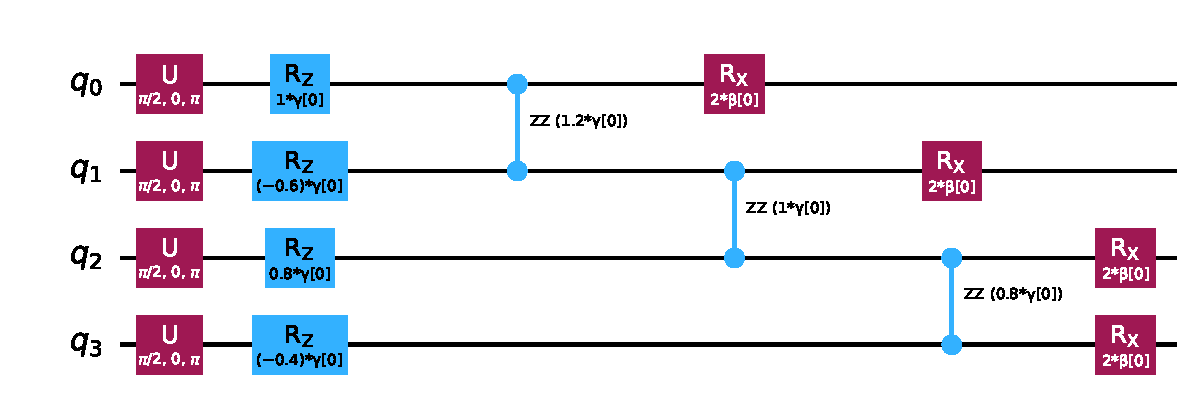
\includegraphics[width=\textwidth]{figures/qaoa_circuit_fibonacci}
\caption{Obwód QAOA ($p=1$) dla czterozmiennowego sąsiedztwa Fibonacciego.
  (Etykiety na rysunku pozostają angielskie.)}
\label{fig:qaoa_fib}
\end{figure}

\subsection{QAOA o ustalonych kątach z offline'ową optymalizacją kątów}
\label{subsec:fixed}
Wariacyjny QAOA re-optymalizuje kąty $(\gamma,\beta)$ dla każdej instancji,
zużywając od dziesiątek do setek wykonań obwodu przed wybraniem jednego ruchu.
Przy szumie NISQ i ciasnym budżecie czasu kwantowego -- plan IBM Open daje
około dziesięciu minut czasu QPU na okno dwudziestoośmiodniowe -- nie jest to
wykonalne wewnątrz metaheurystyki oceniającej tysiące ruchów. Ustalamy zatem
kąty per typ sąsiedztwa i pozyskujemy je offline, jednorazowo. Dla każdego
z czterech sąsiedztw jedna para kątów $(\gamma^\star,\beta^\star)$ jest
optymalizowana na klasycznej symulacji wektora stanu wyczerpującym
przeszukiwaniem dwuwymiarowej siatki w tym przedziale, z lokalnym
doprecyzowaniem, przez minimalizację oczekiwanego kosztu
\begin{equation}
  (\gamma^\star,\beta^\star)
  \;=\; \arg\min_{\gamma,\beta}\
  \langle\gamma,\beta\lvert H_C\rvert\gamma,\beta\rangle,
  \qquad \gamma\in[0,\pi],\ \beta\in[0,\pi/2],
  \label{eq:angleopt}
\end{equation}
uśrednionego po małym zbiorze trenującym reprezentatywnych instancji QUBO tego
sąsiedztwa. Kąty są następnie zamrażane i reużywane dla każdego ruchu tego
sąsiedztwa w czasie działania, więc koszt offline amortyzuje się na całym
przeszukiwaniu, a koszt online na ruch pozostaje jednym wykonaniem obwodu.
Strategia ta opiera się na przenaszalności kątów: dla ustalonego sąsiedztwa
optymalne kąty przy $p=1$ są niemal stałe między instancjami, i na tej
własności projekt się opiera. Jako punkt odniesienia niewymagający trenowania
raportujemy również niezależne od instancji kąty dla $p=1$ dane przez hipotezy
o ustalonych kątach Wurtza i Lykova. Na sprzęcie każdy ruch kosztuje zatem
jedno wykonanie obwodu, co jest bezpośrednim bramkowym odpowiednikiem jednego
wywołania annealera na ruch i stanowi podstawę uczciwego porównania czasu
zegarowego. Pracujemy wszędzie przy $p=1$, czyli na głębokości, którą obecny
sprzęt NISQ wspiera wiarygodnie. Czy większe głębokości się opłacają na
sprzęcie, jest pytaniem na przyszłość: wymaga wielokrotnie więcej wykonań
obwodu, niż pozwala kolejkowane konto z limitem, a zatem lepszego dostępu do
urządzenia, niż mieliśmy tutaj.

\subsection{Sąsiedztwa i ich grafy konfliktów}
\label{subsec:neigh}
Wszystkie cztery sąsiedztwa reużywają swoich QUBO annealingowych i różnią się
wyłącznie wzorcem sprzężeń w warstwie $R_{ZZ}$ w~\eqref{eq:qaoa}, czyli
topologią grafu konfliktów. Sąsiedztwo Adjacent wybiera jedną z $n-1$
transpozycji sąsiednich pod ograniczeniem one-hot, więc każda para zmiennych
koliduje, a jego graf konfliktów jest pełny. Sąsiedztwo Fibonacci karze tylko
kolejne nakładające się wymiany i daje przez to łańcuch tridiagonalny,
najrzadszy z czterech. Sąsiedztwa Dynasearch i Motzkin działają oba na
przedziałach wymiany końców, ale stosują różne reguły konfliktu: Dynasearch
karze każdą parę nakładających się przedziałów, w tym zagnieżdżone, podczas
gdy Motzkin dopuszcza przedziały zagnieżdżone i karze tylko przecięcia oraz
wspólne końce. Graf konfliktów Motzkina jest zatem podgrafem grafu
Dynasearcha i jest od niego ściśle rzadszy, co właśnie stanowi własność
motywującą sąsiedztwo Motzkina. Grafy Adjacent i Dynasearch są gęste
i kompilują się do najgłębszych obwodów, natomiast tridiagonalny łańcuch
Fibonacciego pozostaje najpłytszy; Motzkin leży między nimi, rzadszy niż
Dynasearch, ale znacznie gęstszy niż Fibonacci.
Rysunek~\ref{fig:neigh_circuits} pokazuje przykładowe obwody dla $p=1$ dla
sąsiedztw Adjacent, Dynasearch i Motzkin; obwodem Fibonacciego jest ten
z rys.~\ref{fig:qaoa_fib}. Każda bramka $R_{ZZ}$ odpowiada jednej krawędzi
grafu konfliktów, więc liczbę bramek dwukubitowych odczytuje się wprost
z grafu.

\begin{figure}[p]
\centering
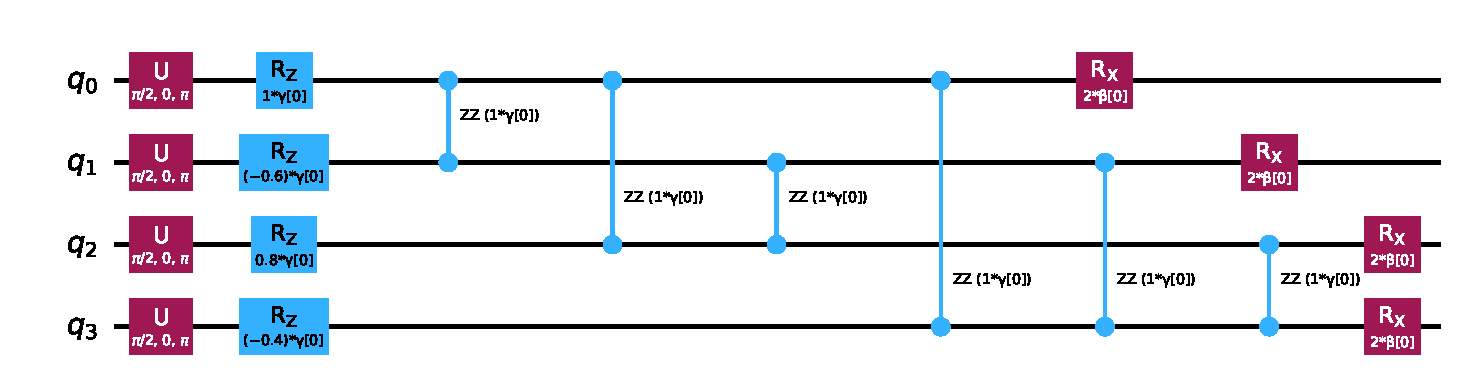
\includegraphics[width=\textwidth]{figures/qaoa_adjacent}\\[0.4ex]
{\footnotesize (a) Adjacent: pełny graf konfliktów (gęsty)}\\[2.2ex]
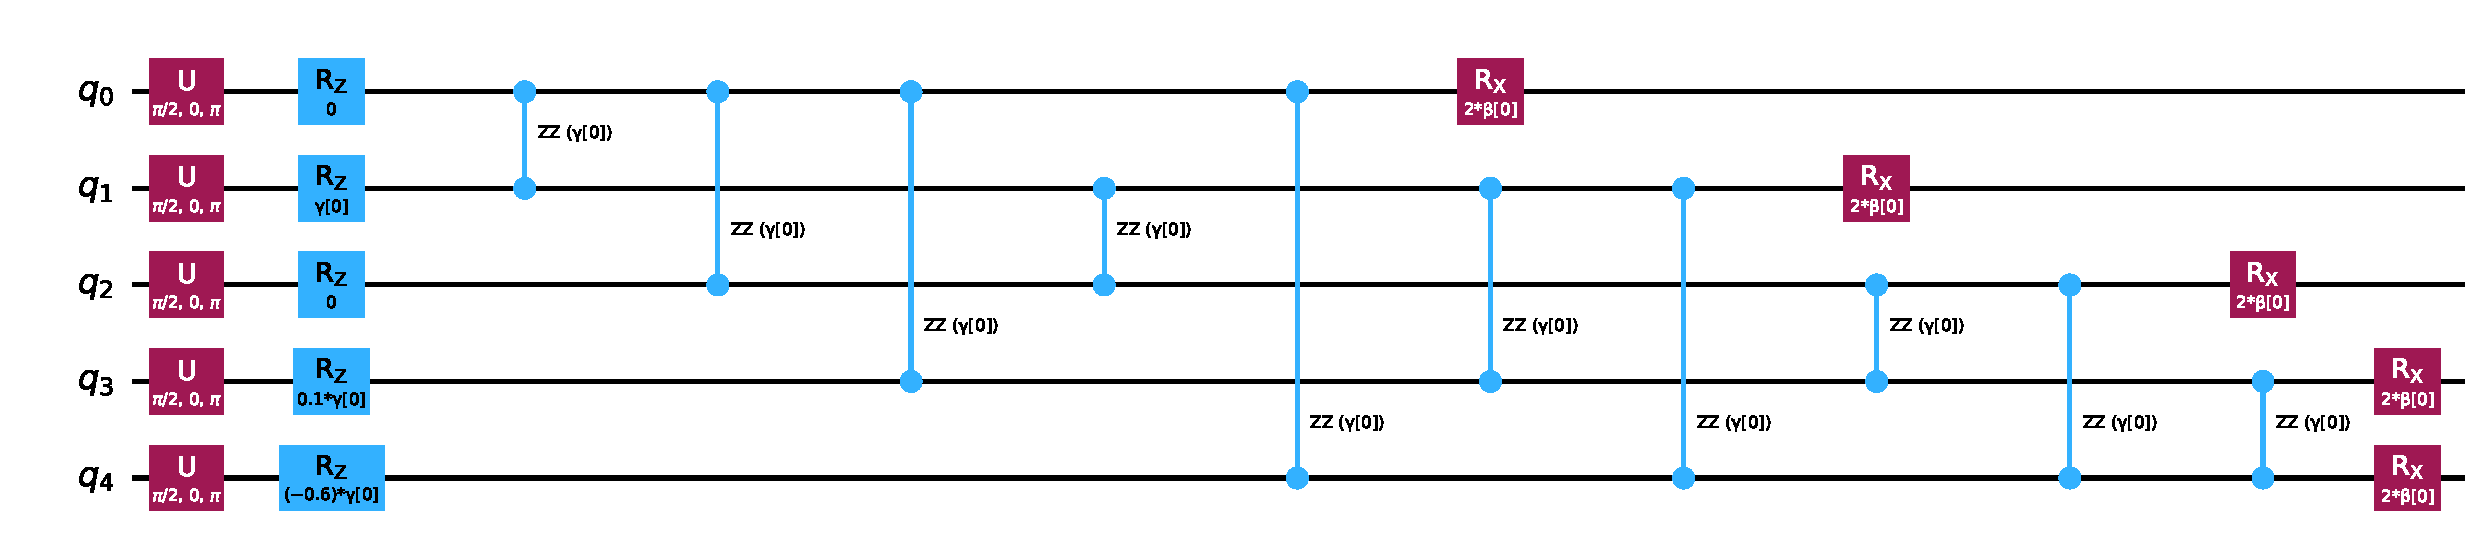
\includegraphics[width=\textwidth]{figures/qaoa_dynasearch}\\[0.4ex]
{\footnotesize (b) Dynasearch: karane wszystkie nakładania przedziałów (gęsty)}\\[2.2ex]
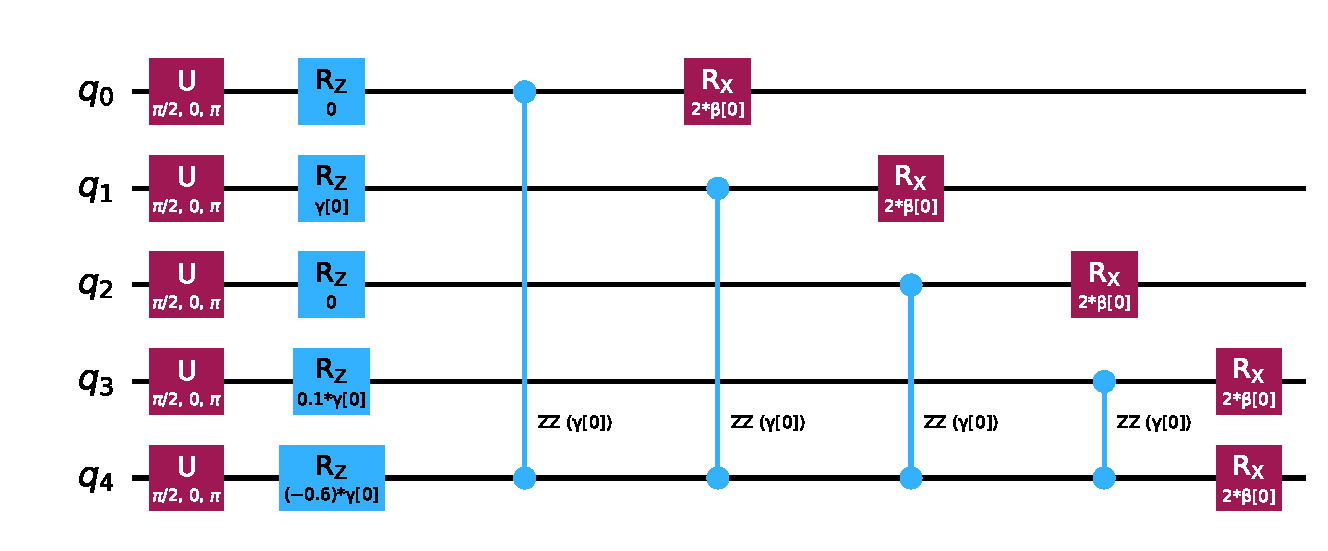
\includegraphics[width=\textwidth]{figures/qaoa_motzkin}\\[0.4ex]
{\footnotesize (c) Motzkin: zagnieżdżanie dopuszczone, karane tylko przecięcia (rzadki)}
\caption{Przykładowe warstwy kosztu i miksera QAOA ($p=1$) dla sąsiedztw
  Adjacent, Dynasearch i Motzkin; Fibonacci na rys.~\ref{fig:qaoa_fib}.
  (Etykiety pozostają angielskie.)}
\label{fig:neigh_circuits}
\end{figure}

\subsection{Kompilacja na różnych mapach sprzężeń}
\label{subsec:depth}
Bramka $R_{ZZ}$ wymaga, by jej dwa kubity były fizycznie sąsiednie, więc na
każdej ustalonej mapie sprzężeń kompilator trasuje pozostałe pary przez sieci
SWAP, które pogłębiają obwód i wprowadzają dodatkowy szum. Głębokość obwodu po
transpilacji odgrywa zatem rolę, jaką na annealerze odgrywa pojemność
embeddingu. Aby oddzielić wpływ mapy sprzężeń od wszystkiego pozostałego,
skompilowaliśmy te same cztery QUBO typu swap-selection, wzięte z pierwszej
instancji Taillarda $20\times5$, na cztery procesory: kratę heavy-hex układu
IBM Heron~r2, kraty kwadratowe układów IQM Crystal~20 i Crystal~54 oraz
architekturę gwiazdy IQM Star~16, w której każdy kubit sprzęga się z jednym
centralnym rezonatorem, a operacja MOVE zajmuje miejsce sieci SWAP. Wszystkie
wielkości brane są przy $p=1$, z oknami po sześć dla gęstych sąsiedztw,
i zsumowane po obwodach jednego ruchu; na Star~16 liczba bramek dwukubitowych
to CZ plus MOVE. Transpilacja nie zużywa czasu urządzenia, więc to porównanie nie
kosztowało limitu.

Tabela~\ref{tab:depth} dopuszcza dwa odczyty. Uszeregowanie czterech
sąsiedztw po głębokości po kompilacji jest takie samo na każdej mapie
sprzężeń, z Fibonaccim wyraźnie poniżej Adjacent i oboma wyraźnie poniżej
Motzkina i Dynasearcha, więc uszeregowanie wykonalności, które obserwowała
linia annealingowa, nie zależy od wyboru sprzętu. Głębokości bezwzględne już
od niego zależą, a heavy-hex jest najmniej korzystną z czterech map, ponieważ
kraty kwadratowe kompilują te same obwody od 1,7 do 2,6 razy płycej.

Wiersz Fibonacciego jest przypadkiem kontrolnym. Jego tridiagonalny QUBO
kompiluje się do czternastu bramek CZ na wszystkich czterech mapach, bo
tridiagonalny graf oddziaływań zanurza się w ścieżkę i nigdzie nie wymaga
trasowania, więc niczego w tym wierszu nie można przypisać urządzeniu.
Architektura gwiazdy znosi trasowanie również dla gęstych sąsiedztw,
obniżając liczbę bramek CZ Dynasearcha z 1668 do 696, ale płaci operacjami
MOVE, które serializują się przez jeden rezonator, i dlatego jej głębokość
wypada między dwiema kratami, a nie poniżej nich. Łączność kupuje liczbę
bramek, nie głębokość.

Dla gęstych sąsiedztw reużywamy dekompozycji okienkowej z linii
annealingowej: rozwiązywanie QUBO na małych, nachodzących na siebie okienkach
utrzymuje każdy obwód per okno na tyle płytki, by wykonał się w budżecie
koherencji sprzętu.

\begin{table}[t]
\centering
\caption{Głębokość po kompilacji $d$ i liczba bramek dwukubitowych dla jednego
  ruchu każdego sąsiedztwa, ze średnią po czterech mapach sprzężeń po prawej.}
\label{tab:depth}
\footnotesize
\setlength{\tabcolsep}{3pt}
\begin{tabular*}{\textwidth}{@{\extracolsep{\fill}}lrrrrrrrr@{\hspace{1.2em}}rr@{}}
\toprule
& \multicolumn{2}{c}{Heron~r2} & \multicolumn{2}{c}{Crystal~20}
& \multicolumn{2}{c}{Crystal~54} & \multicolumn{2}{c}{Star~16}
& \multicolumn{2}{c}{\emph{Średnia}} \\
\cmidrule(lr){2-3}\cmidrule(lr){4-5}\cmidrule(lr){6-7}\cmidrule(lr){8-9}\cmidrule(lr){10-11}
Sąsiedztwo & $d$ & 2q & $d$ & 2q & $d$ & 2q & $d$ & 2q & $d$ & 2q \\
\midrule
Fibonacci  & 58   & 14   & \textbf{22}   & 14   & \textbf{22}   & 14   & 38   & 28            & \emph{35}   & \emph{18} \\
Adjacent   & 337  & 195  & 200  & 153  & \textbf{188}  & 159  & 227  & \textbf{180}  & \emph{238}  & \emph{172} \\
Motzkin    & 2208 & 1455 & 1280 & 1080 & \textbf{1177} & 1077 & 1438 & \textbf{1180} & \emph{1526} & \emph{1198} \\
Dynasearch & 2509 & 1668 & 1466 & 1287 & \textbf{1383} & 1275 & 1758 & \textbf{1438} & \emph{1779} & \emph{1417} \\
\bottomrule
\end{tabular*}
\end{table}

\subsection{Sprzęt i oprogramowanie}
\label{subsec:hw}
Obwody celują w procesor IBM Heron~r2 \texttt{ibm\_fez} (156 kubitów, mapa
sprzężeń heavy-hex z 352 sprzężeniami, natywny zestaw bramek CZ, RZ, SX, X),
dostępny przez Qiskit Runtime (\texttt{qiskit}~2.5.1 z
\texttt{qiskit-ibm-runtime}). Drugi zestaw pomiarów działa na dwóch
procesorach IQM dostępnych przez IQM Resonance: \texttt{garnet} (Crystal~20,
20 kubitów na kracie kwadratowej z 30 sprzężeniami) i \texttt{sirius}
(Star~16, 16 kubitów sprzężonych z jednym centralnym rezonatorem). Oba używają
bramki dwukubitowej CZ z rotacjami jednokubitowymi, a \texttt{sirius} dodaje
operację MOVE kubit--rezonator, więc obwody z rozdziału~\ref{sec:method}
kompilują się na wszystkie trzy urządzenia bez zmian. Harmonogram kątów jest
ustalony z wyprzedzeniem przez kalibrację offline
z podrozdziału~\ref{subsec:fixed}, tak by skąpy czas QPU szedł na pomiar,
a nie na dostrajanie kątów.

% =====================================================================
\section{Wyniki i dyskusja}
\label{sec:results}
Ocena ma dwie części. Pierwsza powtarza protokół linii annealingowej na
procesorze heavy-hex, co stawia wiersze bramkowe obok opublikowanych pomiarów
klasycznych i annealingowych na tych samych instancjach. Druga zmienia mapę
sprzężeń i utrzymuje wszystko pozostałe bez zmian, co poddaje argument
o kompilacji z podrozdziału~\ref{subsec:depth} próbie na sprzęcie, a nie tylko
w kompilatorze. Najpierw podajemy protokół, potem raportujemy każdą z części
po kolei.

\subsection{Protokół oceny}
\label{subsec:protocol}
Idziemy za protokołem okienkowego badania annealingowego, tak by oba zbiory
wyników były bezpośrednio porównywalne: instancje PFSP Taillarda o $n=20$
zadaniach, po dziesięć instancji na konfigurację i te same dolne granice.
W obrębie tego protokołu limit dostępu sięgnął jednej liczby maszyn, więc każdy
raportowany przez nas pomiar dotyczy dziesięciu instancji $m=5$; konfiguracje
$m=10$ i $m=20$ należą do pełnego protokołu omówionego
w rozdziale~\ref{sec:conclusions}. Każde sąsiedztwo napędza pętlę iterowanego przeszukiwania
lokalnego oraz pętlę symulowanego wyżarzania; przy każdym ruchu składane jest
QUBO typu swap-selection z rozdziału~\ref{sec:method} i przekazywane obwodowi
QAOA o ustalonych kątach w miejsce annealera. Jakość rozwiązania raportujemy
jako procentowe odchylenie relatywne
$\mathrm{PRD}=(C_{\max}-\mathrm{LB})/\mathrm{LB}\times100$ od dolnej granicy
Taillarda $\mathrm{LB}$, uśrednione po instancjach przy ustalonym budżecie
czasu zegarowego.

Ruch odczytuje obwód, próbkując go i zwracając wylosowany łańcuch bitów
o najniższej energii \emph{oryginalnego} QUBO. Ten odczyt oparty na energii
jest niezbędny: pojedynczy najbardziej prawdopodobny łańcuch bitów stanu QAOA
o małej głębokości jest zwykle przypisaniem wszystkich zer (nic nie rób) albo
stanem wysokoenergetycznym o wielu jedynkach, a żadne z nich nie jest optimum
QUBO, na którym rozkład się koncentruje.

\subsection{Wykonanie na procesorze heavy-hex}
\label{subsec:hwresults}
Uruchomiliśmy cztery sąsiedztwa bramkowe na \texttt{ibm\_fez} na dziesięciu
instancjach Taillarda $20\times5$ pod obiema metaheurystykami, łącznie
osiemdziesiąt przebiegów, zużywając około 460 sekund czasu QPU. Wszystkie okna
jednego ruchu są zgłaszane jako jedno zadanie, więc ruch kosztuje jedno
zgłoszenie niezależnie od tego, ile okien daje dekompozycja.

Tabela~\ref{tab:rpd_hw} raportuje wynik przy najdłuższym budżecie protokołu,
dziesięciu sekundach. Każdy z osiemdziesięciu przebiegów wykonał dokładnie
jeden ruch i każdy przekroczył swój budżet: zmierzone czasy przebiegu wahały
się od 10 do 288 sekund wobec limitu dziesięciu sekund. Przekroczenie jest
zdominowane przez kolejkowanie i narzut zadania, a nie przez obliczenia,
ponieważ rozliczany czas QPU na ruch to około trzech sekund dla sąsiedztw
liniowych i siedmiu dla okienkowanych. Przebieg wykonuje co najmniej jeden
ruch, a jeden ruch już przekracza najdłuższy budżet, więc żaden krótszy
budżet protokołu również nie dopuści drugiego ruchu. Każda kolumna budżetowa
opisuje zatem to samo obliczenie i nosi tę samą wartość. Raportujemy je jako
takie, oznaczone jako ekstrapolowane z kolumny zmierzonej na mocy tego
argumentu, a nie zmierzone niezależnie.

Adjacent zwraca 25,04 pod obiema metaheurystykami, ponieważ obie pętle startują
z permutacji identycznościowej, a wybór metaheurystyki nie może mieć znaczenia
przed drugim ruchem. Dla pozostałych trzech sąsiedztw wartości ILS i SA różnią
się setnymi punktu procentowego, co jest szumem próbkowania na urządzeniu,
a nie zachowaniem algorytmicznym.

Limit, z którego pochodzą te wiersze, daje dziesięć minut czasu QPU na
miesiąc, co dopuszcza z grubsza jedną kolumnę budżetową przy jednym seedzie.
Jak dużą część kosztu na ruch da się odzyskać agresywniejszym batchowaniem,
płytszymi obwodami albo mniejszą liczbą shotów, pozostaje otwartym pytaniem
inżynierskim. Te same obwody działają na dwóch kolejnych procesorach, o innych
mapach sprzężeń, w podrozdziale~\ref{subsec:arch}.

\subsection{Porównanie z backendami annealingowymi}
\label{subsec:cmp}
Tabela~\ref{tab:cmp} stawia wiersze bramkowe obok klasycznych
i annealingowych pomiarów okienkowego badania na tych samych instancjach i przy
tym samym budżecie, a rys.~\ref{fig:cmp} prowadzi wszystkie cztery backendy
przez cały zakres budżetów.

Na Dynasearchu procesor bramkowy zwraca najniższy PRD z trzech backendów
kwantowych, 22,12 wobec 25,85 dla annealera i 26,24 dla jego wariantu
okienkowanego, i czyni to pod obiema metaheurystykami. Motzkin stawia go
pomiędzy nimi: lepiej niż annealer okienkowany, czyli wariant, z którym
powinien być porównywany, bo oba rozkładają sąsiedztwo na okna, i gorzej niż
pełne sformułowanie annealingowe. Na dwóch sąsiedztwach liniowych wiersze
bramkowe są najsłabsze z trzech, o około pięć punktów.

Część tej luki to opóźnienie dostępu, a nie jakość rozwiązania. Wywołanie
annealera kosztuje rzędu sekundy, więc od dwóch sekund w górę przebiegi
annealingowe zamieniają pozostały budżet na dalsze ruchy, podczas gdy ruch
bramkowy kosztuje około trzydziestu sekund i żaden budżet protokołu nie
dopuszcza drugiego. Przy budżetach do jednej sekundy, gdzie oba backendy
odpowiadają po jednym wywołaniu, wiersze annealingowe i bramkowe dla
sąsiedztw liniowych leżą w granicach kilku dziesiątych punktu od siebie;
porównanie w tabeli~\ref{tab:cmp} jest brane przy budżecie najmniej korzystnym
dla urządzenia bramkowego.

Wszystkie backendy kwantowe pozostają daleko od klasycznych punktów odniesienia
przy tym rozmiarze instancji, tak jak w badaniu annealingowym.

\begin{table}[t]
\centering
\caption{Średni PRD [\%] na \texttt{ibm\_fez} per budżet czasowy (kolumny, ms),
  z odchyleniem standardowym po dziesięciu instancjach w ostatniej kolumnie.}
\label{tab:rpd_hw}
\footnotesize
\renewcommand{\arraystretch}{0.95}
\begin{tabular*}{\textwidth}{@{\extracolsep{\fill}}lrrrrrr@{\hspace{1.2em}}r@{}}
\toprule
ILS & 100 & 500 & 1000 & 2000 & 5000 & 10000 & \emph{std} \\
\midrule
Bramkowy Adjacent   & 25.04 & 25.04 & 25.04 & 25.04 & 25.04 & 25.04 & \emph{10.0} \\
Bramkowy Fibonacci  & 23.41 & 23.41 & 23.41 & 23.41 & 23.41 & 23.41 & \emph{9.2} \\
Bramkowy Dynasearch & \textbf{22.12} & \textbf{22.12} & \textbf{22.12} & \textbf{22.12} & \textbf{22.12} & \textbf{22.12} & \emph{8.0} \\
Bramkowy Motzkin    & 23.12 & 23.12 & 23.12 & 23.12 & 23.12 & 23.12 & \emph{8.0} \\
\midrule
SA & 100 & 500 & 1000 & 2000 & 5000 & 10000 & \emph{std} \\
\midrule
Bramkowy Adjacent   & 25.04 & 25.04 & 25.04 & 25.04 & 25.04 & 25.04 & \emph{10.0} \\
Bramkowy Fibonacci  & 23.48 & 23.48 & 23.48 & 23.48 & 23.48 & 23.48 & \emph{9.0} \\
Bramkowy Dynasearch & \textbf{22.38} & \textbf{22.38} & \textbf{22.38} & \textbf{22.38} & \textbf{22.38} & \textbf{22.38} & \emph{8.7} \\
Bramkowy Motzkin    & 23.59 & 23.59 & 23.59 & 23.59 & 23.59 & 23.59 & \emph{8.1} \\
\bottomrule
\end{tabular*}
\end{table}

\begin{figure}[t]
\centering
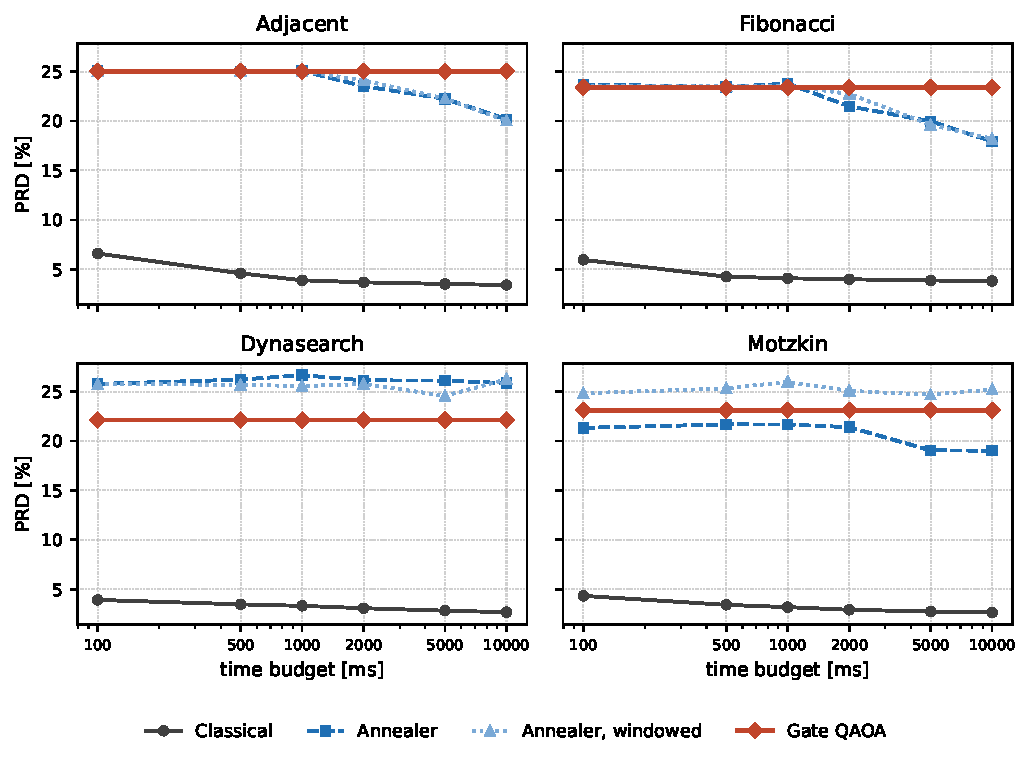
\includegraphics[width=\linewidth]{figures/solver_comparison}
\caption{PRD w funkcji budżetu czasowego dla czterech sąsiedztw pod czterema
  backendami solvera (ILS; SA zachowuje się podobnie). (Etykiety pozostają
  angielskie.)}
\label{fig:cmp}
\end{figure}

\begin{table}[t]
\centering
\caption{PRD [\%] na Taillardzie $20\times5$ przy $t_{\max}=10\,000$\,ms,
  dziesięć instancji. Pogrubienie oznacza najlepszy backend kwantowy dla
  danego sąsiedztwa.}
\label{tab:cmp}
\footnotesize
\setlength{\tabcolsep}{4pt}
\begin{tabular*}{\textwidth}{@{\extracolsep{\fill}}lrrrrrrrr@{}}
\toprule
& \multicolumn{2}{c}{Klasyczny} & \multicolumn{2}{c}{Annealer}
& \multicolumn{2}{c}{Annealer, okn.} & \multicolumn{2}{c}{Bramkowy QAOA} \\
\cmidrule(lr){2-3}\cmidrule(lr){4-5}\cmidrule(lr){6-7}\cmidrule(lr){8-9}
Sąsiedztwo & ILS & SA & ILS & SA & ILS & SA & ILS & SA \\
\midrule
Adjacent    & 3.41 & 6.98 & 20.17 & 20.18 & \textbf{20.03} & \textbf{20.16} & 25.04 & 25.04 \\
Fibonacci   & 3.82 & 9.24 & \textbf{17.94} & \textbf{17.82} & 18.20 & 18.12 & 23.41 & 23.48 \\
Dynasearch  & 2.68 & 3.36 & 25.85 & 26.39 & 26.24 & 26.21 & \textbf{22.12} & \textbf{22.38} \\
Motzkin     & 2.64 & 3.25 & \textbf{19.02} & \textbf{19.10} & 25.22 & 25.15 & 23.12 & 23.59 \\
\midrule
\emph{Średnia} & 3.14 & 5.71 & 20.75 & 20.87 & 22.42 & 22.41 & 23.42 & 23.62 \\
\bottomrule
\end{tabular*}
\end{table}

\subsection{Te same sąsiedztwa na trzech mapach sprzężeń}
\label{subsec:arch}
Argument o głębokości z podrozdziału~\ref{subsec:depth} dotyczy kompilacji,
więc da się go sprawdzić, zmieniając mapę sprzężeń i utrzymując wszystko
pozostałe bez zmian. Powtórzyliśmy protokół pod iterowanym przeszukiwaniem
lokalnym na \texttt{garnet} i na \texttt{sirius}, z tymi samymi QUBO, kątami,
liczbą shotów i startem identycznościowym. Dla Adjacent i Fibonacciego,
których ruch kompiluje się do jednego obwodu, limit pokrył protokół
dziesięcioinstancyjny. Wynikiem jest równość, a nie zgodność. Na wszystkich
dziewięciu instancjach, które mieszczą się w szesnastu kubitach
\texttt{siriusa}, Adjacent zwraca tam ten sam makespan co na
\texttt{ibm\_fez}, instancja po instancji, a obie kolumny dają $25{,}79 \pm 10{,}26$;
różnica względem tabeli~\ref{tab:rpd_hw} to pominięta instancja, a nie
urządzenie. Fibonacci zgadza się na sześciu z tych dziewięciu, a na
pozostałych różni się najwyżej o 0,85 punktu procentowego, przy
$24{,}39 \pm 8{,}99$ przeciw $24{,}43 \pm 9{,}15$. Tridiagonalny lub niemal
tridiagonalny graf konfliktów kompiluje się do obwodu na tyle krótkiego, że
krata heavy-hex ze 156 kubitami i urządzenie z rezonatorem o 16 kubitach
zwracają tę samą odpowiedź, a wiersz Fibonacciego w tabeli~\ref{tab:depth}
mówi dlaczego: oba kompilują go do czternastu bramek CZ.

Gęste sąsiedztwa zachowują się inaczej, a tabela~\ref{tab:arch} raportuje je
na pierwszej instancji, bo dalej limit nie sięgnął. Przebiegi startują
z permutacji identycznościowej, której makespan wynosi tam 1448 wobec dolnej
granicy 1232, czyli PRD 17,53, a kolumna Heron~r2 jest przeliczona z tej jednej
instancji, nie wzięta ze średniej dziesięcioinstancyjnej. Motzkin poprawia się
monotonicznie wraz ze zmianą mapy sprzężeń, łącznie o 3,65 punktu, natomiast
Dynasearch nie podąża za tą kolejnością i wypada najgorzej na kracie
kwadratowej. Jedna instancja nie pozwala odseparować efektu urządzenia od
szumu próbkowania, więc raportujemy ten wiersz tak, jak go zmierzono.

Wzięte razem obie grupy opisują próg, a nie gradient. Adjacent potrzebuje 195
bramek CZ na heavy-hex, 153 na kracie kwadratowej i 90 na urządzeniu
z rezonatorem, a zwraca ten sam makespan na wszystkich trzech. Motzkin spada
w podobnym stosunku na tych samych trzech mapach, z 1455 bramek CZ przez 1080
do 576, i tam PRD obniża się z 16,96 do 13,31. Porównywalna redukcja liczby
bramek nie zmienia więc nic w jednym przypadku, a 3,65 punktu procentowego
w drugim: poniżej pewnej głębokości po kompilacji mapa sprzężeń jest dla
wyniku niewidoczna, a powyżej niej mapa decyduje.

Szesnaście kubitów \texttt{siriusa} jest także wiążącym ograniczeniem już przy
$n=20$, ponieważ szerokość QUBO typu swap-selection waha się od 5 do 18
zmiennych w dziesięciu instancjach i jedna z nich się nie mieści.

\begin{table}[t]
\centering
\caption{PRD [\%] po jednym ruchu na pierwszej instancji Taillarda
  $20\times5$. Pogrubienie oznacza najlepszą mapę sprzężeń; wiersz Adjacent
  jest nieoznaczony, ponieważ wszystkie trzy zgadzają się dokładnie.}
\label{tab:arch}
\footnotesize
\begin{tabular*}{\textwidth}{@{\extracolsep{\fill}}lrrr@{}}
\toprule
Sąsiedztwo & Heron~r2 & Crystal~20 & Star~16 \\
\midrule
Adjacent    & 12.82 & 12.82 & 12.82 \\
Fibonacci   & 12.26 & \textbf{12.01} & \textbf{12.01} \\
Dynasearch  & 12.42 & 15.10 & \textbf{12.09} \\
Motzkin     & 16.96 & 14.85 & \textbf{13.31} \\
\midrule
\emph{Średnia} & 13.62 & 13.70 & 12.56 \\
\bottomrule
\end{tabular*}
\end{table}

% =====================================================================
\section{Wnioski}
\label{sec:conclusions}
Przenieśliśmy pomysł sąsiedztwa-jako-QUBO z kwantowego annealera na model
bramkowy. Jedna macierz swap-selection napędza dowolne z obu urządzeń, więc
cztery struktury sąsiedztw, ich kary i odwzorowanie z powrotem na permutację
są wspólne, a zmienia się tylko solver; zamrożenie kątów QAOA offline redukuje
koszt online do jednego wykonania obwodu na ruch, czyli budżetu, jaki zużywa
wywołanie annealera. Analiza wskazuje głębokość obwodu po kompilacji jako
bramkowy odpowiednik pojemności embeddingu: graf konfliktów przekraczający
łączność annealera trasuje się także w głęboki, zaszumiony obwód, więc oba
paradygmaty porządkują sąsiedztwa po wykonalności w ten sam sposób, z powodów
pozostających bez związku. Skompilowanie tych samych czterech QUBO na kratę
heavy-hex, dwie kraty kwadratowe i urządzenie z rezonatorem nie zmienia tego
uszeregowania, a przesuwa głębokości bezwzględne dwukrotnie, co czyni argument
twierdzeniem o kompilacji, a nie o topologii jednego producenta, przy czym
heavy-hex jest najmniej korzystną z czterech. Na sprzęcie konsekwencją jest
próg, a nie trend: sąsiedztwa kompilujące się do krótkich obwodów zwracają ten
sam makespan na procesorze heavy-hex ze 156 kubitami i na urządzeniu
z rezonatorem o 16 kubitach, instancja po instancji.

To, co udało się zmierzyć, jest ograniczone przydziałem, a nie metodą. Każdy
przebieg wykonał jeden ruch niezależnie od budżetu, bo ruch kosztuje około
trzydziestu sekund czasu zegarowego wobec trzech do siedmiu sekund obliczeń,
a ten sam ruch zajmuje dwanaście sekund na mniej obciążonym procesorze, więc
ta liczba mierzy kontencję; wymiar czasowy protokołu zapada się zatem. Pełny
protokół linii annealingowej, dziesięć instancji przy pięciu seedach na sześciu
budżetach dla obu metaheurystyk, kosztuje około 550 kredytów czasu urządzenia
na procesor przy zmierzonych przez nas stawkach, przeciw trzydziestu
z przydziału miesięcznego, i zamierzamy go przeprowadzić po uzyskaniu
większego przydziału, na tych samych instancjach, seedach i budżetach oraz na
każdej z map sprzężeń. Skalowanie po $n$ niesie koszt własny, bo rozliczanie
idzie za liczbą obwodów, a nie za ich głębokością: jeden ruch gęstego
sąsiedztwa potrzebuje sześciu obwodów przy $n=20$ i 166 przy $n=500$, więc
cena rośnie liniowo z rozmiarem instancji, podczas gdy jedno wywołanie
annealera obsługuje cały QUBO aż do granicy embeddingu. Jedno pytanie
zostawiamy otwarte i jest ono metodologiczne, bo ścisłe kryterium czasu
zegarowego dolicza oczekiwanie w kolejce do algorytmu, choć to oczekiwanie
waha się o rząd wielkości między identycznymi zgłoszeniami.

\bigskip
\noindent\footnotesize
\emph{Uwaga techniczna.} Cytowania zostały w tym tłumaczeniu pominięte
w tekście ciągłym; pełna, numerowana bibliografia znajduje się w wersji
angielskiej (\texttt{main.tex}), która jest wersją wiążącą. Rysunki są
reużywane bez zmian, więc etykiety na diagramach obwodów i na wykresie
porównawczym pozostają angielskie.


\section*{Podziękowania}
\noindent Autorzy korzystali z dużego modelu językowego jako pomocy
redakcyjnej i przy przeglądzie kodu w trakcie przygotowania manuskryptu;
wyniki, ich interpretacja i tekst końcowy są własne autorów.

\normalsize
\section*{Bibliografia}
\noindent\footnotesize Wykaz przeniesiony bez zmian z wersji angielskiej;
numeracja jest z nią zgodna. Autocytowania pokazano z nazwiskami,
w odróżnieniu od wersji angielskiej, która idzie do recenzji blind.
\normalsize

\begin{thebibliography}{22}

\bibitem{ahuja2002}
Ahuja, R.K., Ergun, \"{O}., Orlin, J.B., Punnen, A.P.: A survey of very
large-scale neighborhood search techniques. Discrete Appl. Math.
\textbf{123}(1--3), 75--102 (2002).
\url{https://doi.org/10.1016/S0166-218X(01)00338-9}

\bibitem{amaro2022}
Amaro, D., Rosenkranz, M., Fitzpatrick, N., Hirano, K., Fiorentini, M.:
A case study of variational quantum algorithms for a job shop scheduling
problem. EPJ Quantum Technol. \textbf{9}, 5 (2022).
\url{https://doi.org/10.1140/epjqt/s40507-022-00123-4}

\bibitem{chamberland2020}
Chamberland, C., Zhu, G., Yoder, T.J., Hertzberg, J.B., Cross, A.W.:
Topological and subsystem codes on low-degree graphs with flag qubits.
Phys. Rev. X \textbf{10}, 011022 (2020).
\url{https://doi.org/10.1103/PhysRevX.10.011022}

\bibitem{congram2002}
Congram, R.K., Potts, C.N., van de Velde, S.L.: An iterated dynasearch
algorithm for the single-machine total weighted tardiness scheduling
problem. INFORMS J. Comput. \textbf{14}(1), 52--67 (2002).
\url{https://doi.org/10.1287/ijoc.14.1.52.7712}

\bibitem{farhi2014qaoa}
Farhi, E., Goldstone, J., Gutmann, S.: A quantum approximate
optimization algorithm. arXiv:1411.4028 (2014).
\url{https://doi.org/10.48550/arXiv.1411.4028}

\bibitem{galda2021}
Galda, A., Liu, X., Lykov, D., Alexeev, Y., Safro, I.: Transferability of
optimal QAOA parameters between random graphs. In: 2021 IEEE
International Conference on Quantum Computing and Engineering (QCE),
pp.\ 171--180. IEEE (2021).
\url{https://doi.org/10.1109/QCE52317.2021.00034}

\bibitem{garey1976}
Garey, M.R., Johnson, D.S., Sethi, R.: The complexity of flowshop and
jobshop scheduling. Math. Oper. Res. \textbf{1}(2), 117--129 (1976).
\url{https://doi.org/10.1287/moor.1.2.117}

\bibitem{kadowaki1998}
Kadowaki, T., Nishimori, H.: Quantum annealing in the transverse Ising
model. Phys. Rev. E \textbf{58}(5), 5355--5363 (1998).
\url{https://doi.org/10.1103/PhysRevE.58.5355}

\bibitem{kirkpatrick1983}
Kirkpatrick, S., Gelatt, C.D., Vecchi, M.P.: Optimization by simulated
annealing. Science \textbf{220}(4598), 671--680 (1983).
\url{https://doi.org/10.1126/science.220.4598.671}

\bibitem{li2019}
Li, G., Ding, Y., Xie, Y.: Tackling the qubit mapping problem for
NISQ-era quantum devices. In: Proceedings of the 24th International
Conference on Architectural Support for Programming Languages and
Operating Systems (ASPLOS), pp.\ 1001--1014. ACM (2019).
\url{https://doi.org/10.1145/3297858.3304023}

\bibitem{lourenco2003}
Louren\c{c}o, H.R., Martin, O.C., St\"{u}tzle, T.: Iterated local search.
In: Glover, F., Kochenberger, G.A. (eds.) Handbook of Metaheuristics,
pp.\ 320--353. Kluwer, Boston (2003).
\url{https://doi.org/10.1007/0-306-48056-5_11}

\bibitem{lucas2014ising}
Lucas, A.: Ising formulations of many NP problems. Front. Phys.
\textbf{2}, 5 (2014). \url{https://doi.org/10.3389/fphy.2014.00005}

\bibitem{neh1983}
Nawaz, M., Enscore, E.E., Ham, I.: A heuristic algorithm for the
m-machine, n-job flow-shop sequencing problem. Omega \textbf{11}(1),
91--95 (1983). \url{https://doi.org/10.1016/0305-0483(83)90088-9}

\bibitem{preskill2018}
Preskill, J.: Quantum computing in the NISQ era and beyond. Quantum
\textbf{2}, 79 (2018). \url{https://doi.org/10.22331/q-2018-08-06-79}

\bibitem{ruizmaroto2005}
Ruiz, R., Maroto, C.: A comprehensive review and evaluation of
permutation flowshop heuristics. Eur. J. Oper. Res. \textbf{165}(2),
479--494 (2005). \url{https://doi.org/10.1016/j.ejor.2004.04.017}

\bibitem{taillard1993}
Taillard, \'{E}.: Benchmarks for basic scheduling problems. Eur. J. Oper.
Res. \textbf{64}(2), 278--285 (1993).
\url{https://doi.org/10.1016/0377-2217(93)90182-M}

\bibitem{venturelli2015}
Venturelli, D., Marchand, D.J.J., Rojo, G.: Quantum annealing
implementation of job-shop scheduling. arXiv:1506.08479 (2015).
\url{https://doi.org/10.48550/arXiv.1506.08479}

\bibitem{wojewodzki2026bpasts}
\ifblind
[Authors omitted for blind review]: Classical and quantum neighborhoods
evaluation in iterated local search and simulated annealing for the
permutation flow shop problem. Bull. Pol. Acad. Sci. Tech. Sci.
(under review, 2026)
\else
Wojew\'{o}dzki, R., Bo\.{z}ejko, W.: Classical and quantum neighborhoods
evaluation in iterated local search and simulated annealing for the
permutation flow shop problem. Bull. Pol. Acad. Sci. Tech. Sci.
(under review, 2026)
\fi

\bibitem{wojewodzki2026soco}
\ifblind
[Authors omitted for blind review]: Motzkin neighborhood evaluation in
iterated local search and simulated annealing for the permutational
flow shop problem. In: SOCO 2026, CCIS, vol.\ 3046, pp.\ 144--155.
Springer (2026)
\else
Wojew\'{o}dzki, R., Bo\.{z}ejko, W.: Motzkin neighborhood evaluation in
iterated local search and simulated annealing for the permutational
flow shop problem. In: SOCO 2026, CCIS, vol.\ 3046, pp.\ 144--155.
Springer (2026). \url{https://doi.org/10.1007/978-3-032-29254-4_12}
\fi

\bibitem{wojewodzki2026windowed}
\ifblind
[Authors omitted for blind review]: Scalable quantum neighborhood search
for the permutation flow shop problem via windowed QUBO decomposition.
Comput. Oper. Res. (under review, 2026)
\else
Wojew\'{o}dzki, R., Bo\.{z}ejko, W.: Scalable quantum neighborhood search
for the permutation flow shop problem via windowed QUBO decomposition.
Comput. Oper. Res. (under review, 2026)
\fi

\bibitem{wurtz2021fixed}
Wurtz, J., Lykov, D.: Fixed-angle conjectures for the quantum approximate
optimization algorithm on regular MaxCut graphs. Phys. Rev. A
\textbf{104}, 052419 (2021).
\url{https://doi.org/10.1103/PhysRevA.104.052419}

\bibitem{zhou2020}
Zhou, L., Wang, S.-T., Choi, S., Pichler, H., Lukin, M.D.: Quantum
approximate optimization algorithm: performance, mechanism, and
implementation on near-term devices. Phys. Rev. X \textbf{10}, 021067
(2020). \url{https://doi.org/10.1103/PhysRevX.10.021067}

\end{thebibliography}

\end{document}
